% 2010 年江西卷理科第 16 题：三棱锥 O-ABC（OA、OB、OC 两两垂直）。
% 来源 PDF：普通高考/2010/2010江西理.pdf，SHA-256 994a56c33da151e22af3fabe292d1b5b193866dfc35773a4431e6dfc8a0cc934。
% 原页：第 1 页（A3 三栏）第 2 栏下部，书页码 607。
% 重绘依据：照原页，O 在上，A 左下，B 右下，C 在右侧中部；OA、OB、OC 为三条两两垂直的棱，
%   可见棱 OA、OB、OC、AB、BC 画实线，被面 OAB 遮挡的棱 AC 画虚线。
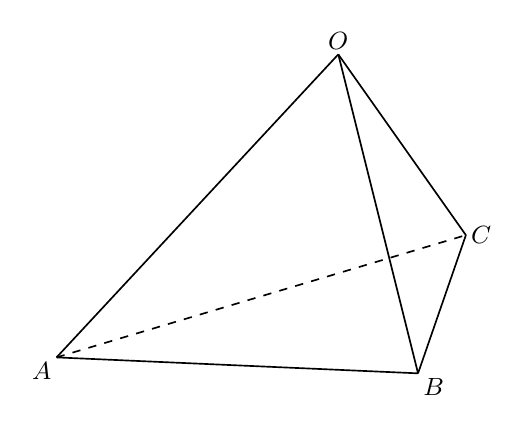
\begin{tikzpicture}[semithick, scale=1.35, every node/.style={inner sep=1.6pt, font=\small}]
  \coordinate (O) at (0.35,1.85);
  \coordinate (A) at (-2.3,-1.0);
  \coordinate (B) at (1.1,-1.15);
  \coordinate (C) at (1.55,0.15);
  \draw (O) -- (A);
  \draw (O) -- (B);
  \draw (O) -- (C);
  \draw (A) -- (B);
  \draw (B) -- (C);
  \draw[dashed] (A) -- (C);
  \node[above] at (O) {$O$};
  \node[below left] at (A) {$A$};
  \node[below right] at (B) {$B$};
  \node[right] at (C) {$C$};
\end{tikzpicture}
